\chapter{Design dei Benchmark e Risultati}
\label{sec:benchmark}

In questo capitolo verranno presentati i benchmark sviluppati per confrontare le performance delle soluzioni basate su CUDA e Vulkan. Verranno, inoltre, presentati i risultati ottenuti e il processo di generazione dei dati.

\section{Benchmark}

Sono stati sviluppati due tipi di benchmark: uno per la somma di vettori e uno per la moltiplicazione di matrici sparse. Le misurazioni hanno tenuto conto sia del tempo di esecuzione su GPU che del tempo di trasferimento dei dati tra tra memoria host e device. I calcoli sono stati eseguiti per tre tipi di dato: \verb|uint|, \verb|float| e \verb|double| (rispettivamente \verb|u32|, \verb|f32| e \verb|f64| in Rust). Questo ha permesso di capire come codice ottimizzato in modo diverso, in base al tipo di dato, da CUDA o Vulkan intacchi le performance. 

La suite è stata eseguita, per tutte le implementazioni, su una macchina con la stessa versione dei driver, per garantire la coerenza dei risultati. In fig. \ref{fig:macchina} sono mostrate le caratteristiche della GPU della macchina. I componenti principali del sistema ibrido sono: CPU Intel Xeon Platinum 8259CL e GPU NVIDIA Tesla T4 Tensor da 16 GB di memoria GDDR6.

\begin{figure}[ht]
    \centering
    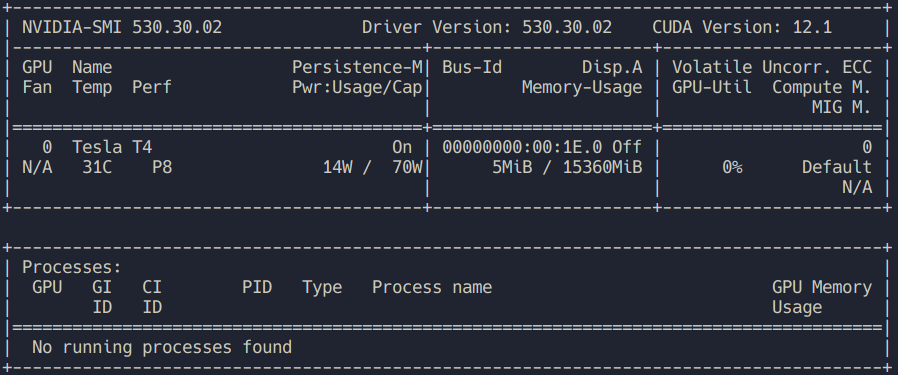
\includegraphics[width=.9\linewidth]{images/chapter4/macchina.png}
    \caption{Specifiche e driver della GPU su cui sono stati eseguiti i benchmark}
    \label{fig:macchina}
\end{figure}

Mentre all'inizio si era pensato di includere anche una versione dei benchmark su CPU, si è poi deciso di scartarli, in quanto non rilevanti per il confronto tra le due soluzioni e poiché i tempi di esecuzione dell'intera suite erano già molto elevati. 

La compilazione di entrambi gli eseguibili è stata ottimizzata, tramite flag dei rispettivi compilatori \ref{lis:comp_flags}, in modo da ottenere il massimo delle performance. Sebbene questa accortezza non intacchi le prestazioni su GPU, è comunque necessaria per avere throughput massimo della CPU per il trasferimento dei dati dalla memoria host a quella device e viceversa.

\vspace{5mm}
\begin{lstlisting}[language=bash, caption=Flag di compilazione CUDA e Rust, label=lis:comp_flags]
# Makefile CUDA
nvcc main.cu -o microbench_cuda -O3 && strip microbench_cuda

# Cargo.toml
[profile.release]
strip = true
panic = "abort"
opt-level = 3
\end{lstlisting}
\vspace{5mm}

I tempi di esecuzione sono stati calcolati mediante funzioni fornite dalla libreria standard di entrambi i linguaggi, e sono stati ricalcolati più volte per ottenere una media più accurata. Per Vulkan si è usata la struct \verb|std::time::Instant| di Rust, mentre per CUDA si è sviluppato un timer che incorpora le funzioni \verb|cudaEventCreate| e \verb|cudaEventElapsedTime|, mostrato in \ref{lis:cuda_timer}, per implementare API simili a quelle usate in Rust. 

I tempi risultanti sono stati poi stampati su standard output specificando il tipo di benchmark di riferimento: ad esempio \verb|SUM VEC and COPY to host: 0.0000 ms| oppure \verb|MUL MAT and COPY to host: 0.0000 ms|. Questo ha permesso di verificare che i tempi di esecuzione fossero coerenti con le operazioni eseguite e di poter confrontare i risultati ottenuti con quelli attesi. 

\newpage
\vspace{5mm}
\begin{lstlisting}[language=C++, caption=Timer CUDA, label=lis:cuda_timer]
class Timer {
  cudaEvent_t start, stop;
  float elapsedTime = 0.0;

 public:
  void startTimer() {
    cudaEventCreate(&start);
    cudaEventRecord(start, 0);
  }

  void stopTimer() {
    cudaEventCreate(&stop);
    cudaEventRecord(stop, 0);
    cudaEventSynchronize(stop);
  }

  float calculateElapsed() {
    cudaEventElapsedTime(&elapsedTime, start, stop);
    return elapsedTime;
  }
};
\end{lstlisting}
\vspace{5mm}


Inoltre ogni eseguibile accetta da linea di comando dei parametri per specificare la dimensione di vettori e matrici con cui eseguire i calcoli, il numero di iterazioni e il tipo di dato da testare \ref{lis:cmd_param}.

Il parametro \verb|vec_exp| indica la grandezza dei vettori: viene eseguita la somma su due vettori di $2^{vec\_exp}$ elementi, con \verb|vec_exp=29| per i tipi di dato \verb|uint| e \verb|float| e \verb|vec_exp=28| per il dato \verb|double| (tutti vettori da 2GB, dato che \verb|double| ha il doppio dei bit di un \verb|uint| e \verb|float|). Durante i test ci si è accorti che aumentando la dimensione dei vettori oltre questo valore, il programma dava errore di allocazione di memoria, dovuto al fatto che raddoppiando il numero di elementi raddoppiavano conseguentemente i thread da eseguire e quindi l'overhead dovuto al caricamento del contesto. Inoltre questa dimensione è sufficiente per testare ler performance della GPU, senza aumentare eccessivamente i tempi di esecuzione.

\vspace{5mm}
\begin{lstlisting}[language=bash, caption=Esecuzione benchmark, label=lis:cmd_param]
# CUDA
./microbench_cuda $vec_exp $dim_m $dim_n $dim_k $num_run $dtype

# Rust
./microbench_vulkan $vec_exp $dim_m $dim_n $dim_k $num_run $dtype
\end{lstlisting}
\vspace{5mm}

Per le matrici, invece, i tre elementi \verb|$dim_m, $dim_n, $dim_k|, indicano la dimensione di righe e colonne, quindi matrici di dimensione $M \times N$ e $N \times K$, che producono è una matrice grande $M \times K$. Nonostante le matrici QUBO siano quadrate e triangolari superiori, si è scelto di generalizzare il più possibile il benchmark, e quindi testare il prodotto di due matrici sparse. Quello che ci si aspetta è che, per la risoluzione di matrici QUBO di dimensioni paragonabili, i tempi d'esecuzione siano leggermente ridotti poiché, come si è visto in \ref{lis:qubo_sol}, si accede solo alla diagonale superiore, eseguendo però due motiplicazioni sui dati. I valori usati per i benchmark sono \verb|dim_m=dim_k=1024| e \verb|dim_n=4096|. Le dimensioni sono state scelte in modo da mantenere un compromesso tra dimensioni e tempo di esecuzione, in modo da poter eseguire un numero di iterazioni sufficiente per ottenere una media accurata: durante i test ci si è accorti che anche aumentando di dimensioni la differenza del tempo di esecuzione tra CUDA e Vulkan rimaneva pressoché invariata, ma aumentava considerevolmente il tempo di esecuzione. 

Il parametro \verb|$num_run| indica il numero di iterazioni da eseguire per calcolare la media dei tempi di esecuzione. Infine, \verb|$dtype| indica il tipo di dato da usare per i calcoli, e può essere \verb|uint|, \verb|float| o \verb|double|.

Per automatizzare il processo di benchmarking, si è scritto uno script Python che lancia some sotto-processi gli eseguibili dei benchmark e, leggendo tramite pipe lo standard output del programma, salva i risultati di ogni iterazione in un file json. Infine, lo script riassume i risultati su un file CSV calcolando le medie dei tempi e produce un grafico che mostra i tempi di esecuzione evidenziando la media e gli outlier.

\begin{figure}[ht]
  \centering
  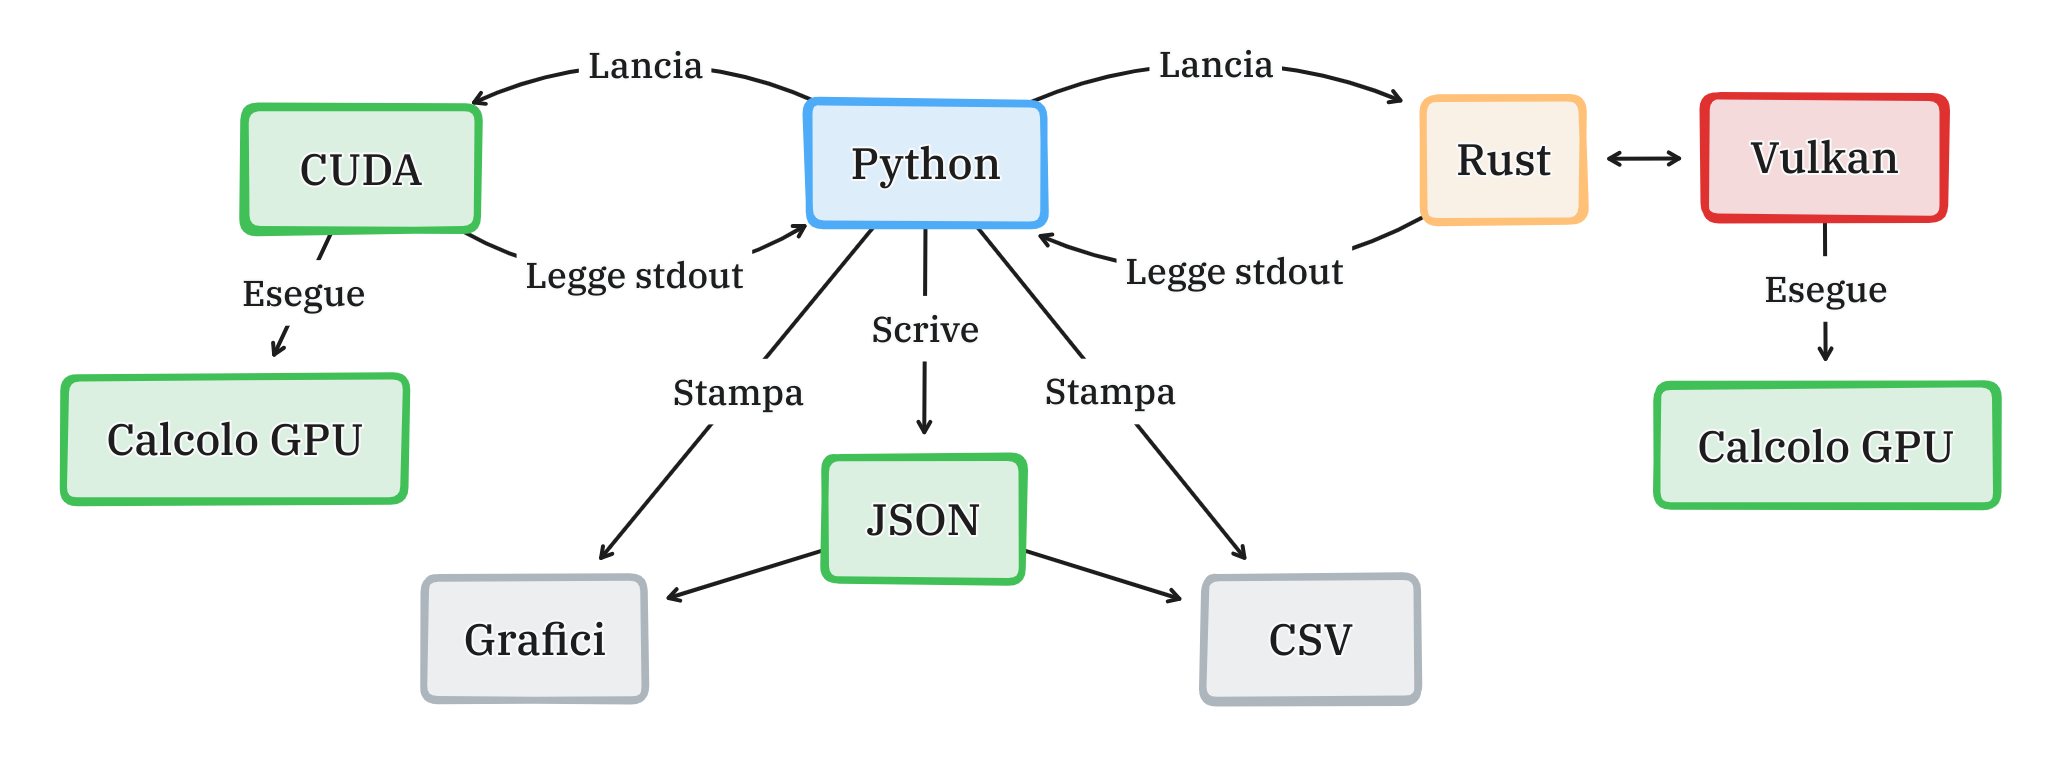
\includegraphics[width=1\linewidth]{images/chapter4/arch_bench.png}
  \caption{Schema logico del processo di benchmarking}
  \label{fig:arch_bench}
\end{figure}

% generazione e verifica dei dati

I dati contenuti nei vettori e nelle matrici sono stati generati casualmente a ogni esecuzione, in modo da garantire che i dati siano sempre diversi e non influenzino in alcun modo i risultati. Il risultato delle operazioni di kernel e shader viene verificato tramite funzioni \verb|assert| presenti nei linguaggi usati. Le funzioni di somma di vettori e moltiplicazione di matrici vengono quindi eseguite su CPU e confrontate con i risultati ottenuti dall'esecuzione su GPU, in modo da garantire che le operazioni siano corrette. A questo proposito c'è da specificare che, per quanto riguarda la moltiplicazione di matrici di tipo \verb|float| e \verb|double|, la funzione di confronto è scritta in modo da eseguire su CPU una \gls{FMA}, in quanto questa operazione è eseguita in modo automatico e trasparente su GPU e influenza l'approssimazione dei risultati e quindi la verifica della correttezza. 

% spiegare FMA

La FMA è un'operazione che consente di eseguire una moltiplicazione tra due operandi e di aggiungere un terzo operando al risultato, in un unico passaggio. Questo approccio offre diversi vantaggi, inclusi una maggiore efficienza computazionale, una riduzione della latenza e un aumento della precisione. Le GPU moderne incorporano unità hardware specializzate per eseguire operazioni FMA in modo efficiente, contribuendo così alla loro capacità di elaborazione ad alte prestazioni \cite[]{NVIDIA:fma}. I moderni processori x86 e ARM incorporano anche unità FMA, ma non sempre sono in grado di eseguire operazioni FMA in modo efficiente come le GPU. Sia CUDA che Rust espongono funzioni nella libreria standard per eseguire operazioni FMA, e quindi, usandole, è stato possibile confrontare in modo preciso i risultati ottenuti su CPU con quelli ottenuti su GPU.

% spiegare programmazione generica

Per diminuire il boilerplate e la quantità di codice da scrivere per ogni benchmark, le funzioni sono state scritte usando la programmazione generica, in modo da poter eseguire le stesse operazioni sui diversi tipi di dato. Questo ha permesso di scrivere una sola volta il codice per la somma di vettori e la moltiplicazione di matrici, e di poterlo eseguire su tutti e tre i tipi di dato. In CUDA si è sfruttato i \verb|template|, come mostrato in \ref{lis:generic_cuda}, sia per le funzioni kernel che per le funzioni host che le richiamano. Le funzioni vengono generate, a tempo di compilazione, per ogni tipo di dato effettivamente usato, ed è quindi il compilatore che si occupa di generare il codice specifico per i dati. 

\vspace{5mm}
\begin{lstlisting}[language=C++, caption=Programmazione generica in CUDA, label=lis:generic_cuda]
template <typename T>
__global__ void vecAddKernel(const T *vec_a, const T *vec_b, 
    T *res, const uint n) { ... }
template <typename T>
__global__ void matrixMulKernel(const T *mat_a, const T *mat_b, 
    T *res, const uint m, const uint n, const uint k) { ... }

template <typename T>
void vecAdd(const T *h_data_a, const T *h_data_b, 
    const uint len) { 
  ...
  vecAddKernel<<<...>>>(vec_a, vec_b, res_data, len);
  ...
}

template <typename T>
void matMul(const T *h_mat_a, const T *h_mat_b, 
    const uint m, const uint n, const uint k) { 
  ... 
  matrixMulKernel<<<...>>>(mat_a, mat_b, res, m, n, k);
  ...
}

template <typename T>
void benchmark(const uint len, const uint dim_m, 
    const uint dim_n, const uint dim_k, const uint num_run) {
  ...
  for (uint i = 0; i < num_run; i++) {
    vecAdd(vec_a, vec_b, len);
    ...
    matMul(mat_a, mat_b, dim_m, dim_n, dim_k);
  }
  ...
}

int main( ... ) {
  ...
  if (strcmp(dtype, "uint") == 0) {
    benchmark<uint>(len, dim_m, dim_n, dim_k, num_run);
  } else if (strcmp(dtype, "float") == 0) {
    benchmark<float>(len, dim_m, dim_n, dim_k, num_run);
  } else if (strcmp(dtype, "double") == 0) {
    benchmark<double>(len, dim_m, dim_n, dim_k, num_run);
  } else {
    return -1;
  }
  ...
}
\end{lstlisting}
\vspace{5mm}

Per quanto riguarda Vulkan, dato che GLSL non supporta la programmazione generica, si è dovuto scrivere tre versioni di ogni compute shader, una per ogni tipo di dato. Tramite la creazione di \verb|enum| specifici e il \verb|pattern matching| di Rust si è comunque riusciti a generalizzare abbastanza le funzioni dei benchmark evitando di scrivere manualmente tre versioni diverse. In \ref{lis:generic_glsl} è mostrato l'approccio usato per ovviare alla mancanza di generics in GLSL, da notare che \verb|ld| è il modulo con cui vengono caricati gli shader, tramite macro a compile time, come visto in \ref{lis:rust_macro}.

\newpage
\vspace{5mm}
\begin{lstlisting}[language=Rust, caption=Loading shader con enum, label=lis:generic_glsl]
#[allow(non_camel_case_types)]
#[derive(Clone, Copy)]
pub enum Type {
  uint,
  float,
  double,
}

pub enum Operation {
  Sum(Type),
  Mul(Type),
}

impl Operation {
  pub fn load_shader(&self, device: Arc<Device>)
    -> Result<Arc<ShaderModule>> {
    let shader = match self {
      Operation::Sum(Type::uint) => ld::sum_uint::load(device)?,
      Operation::Sum(Type::float) => ld::sum_float::load(device)?,
      Operation::Sum(Type::double) => ld::sum_double::load(device)?,
      Operation::Mul(Type::uint) => ld::mul_uint::load(device)?,
      Operation::Mul(Type::float) => ld::mul_float::load(device)?,
      Operation::Mul(Type::double) => ld::mul_double::load(device)?,
    };

    Ok(shader)
  }
}
\end{lstlisting}
\vspace{5mm}

Per quanto riguarda le operazioni sui dati in \ref{lis:generic_rust} è mostrato come usando il \textit{composition pattern} in Rust è possibile implementare il tratto \verb|Add| usato per la somma dei vettori e implementare la FMA per la moltiplicazione delle matrici. Il resto della logica rimane invariata rispetto a CUDA, con una funzione \verb|benchmark::<T>(..., Type::T)| che specializza il tipo di dato ed esegue tutte le operazioni necessarie.

\newpage
\vspace{5mm}
\begin{lstlisting}[language=Rust, caption=Programmazione generica in Rust, label=lis:generic_rust]
#[allow(non_camel_case_types)]
#[derive(PartialEq, Debug, Clone, Copy)]
pub enum DataType {
  uint(u32),
  float(f32),
  double(f64),
}

impl Add for DataType {
  type Output = Self;

  fn add(self, rhs: Self) -> Self::Output {
    match (self, rhs) {
      (Self::uint(x), Self::uint(y)) => Self::uint(x + y),
      (Self::float(x), Self::float(y)) => Self::float(x + y),
      (Self::double(x), Self::double(y)) => Self::double(x + y),
      _ => unreachable!(),
    }
  }
}

impl DataType {
  pub fn fma(a: Self, b: Self, c: Self) -> Self {
    match (a, b, c) {
      (Self::uint(a), Self::uint(b), Self::uint(c)) => {
        Self::uint(a * b + c)
      }
      (Self::float(a), Self::float(b), Self::float(c)) => {
        Self::float(a.mul_add(b, c))
      }
      (Self::double(a), Self::double(b), Self::double(c)) => {
        Self::double(a.mul_add(b, c))
      }
      (Self::float(a), Self::float(b), Self::uint(c)) => {
        Self::float(a.mul_add(b, c as f32))
      }
      (Self::double(a), Self::double(b), Self::uint(c)) => {
        Self::double(a.mul_add(b, c as f64))
      }
      _ => unreachable!(),
    }
  }
}
\end{lstlisting}
\vspace{5mm}

% todo: row major e column major

\newpage
\section{Dati}

In tabella \ref{table:cuda_bench} sono riassunti i risultati ottenuti con CUDA, mentre in tabella \ref{table:vulkan_bench} sono mostrati i risultati ottenuti con Vulkan. Le misure sono fornite in millisecondi e arrotondati a 3 decimali.

% tabelle con le medie dei risultati

\vspace{5mm}
\begin{table}[ht]
  \centering
  \renewcommand{\arraystretch}{1.3}

  \begin{tabular}[t]{ ||l *{3}{ || r }|| }
    \hline \hline
    \multicolumn{4}{||c||}{uint} \\
    \hline
    & min  & max  & mean  \\
    \hline
    SUM VEC and NO COPY & 25.213 & 25.115 & 25.139 \\
    SUM VEC and COPY & 246.253 & 224.671 & 234.274 \\
    MUL MAT and NO COPY & 12.641 & 12.568 & 12.622 \\
    MUL MAT and COPY & 31.283 & 31.048 & 31.132 \\  
    \hline

    \hline \hline
    \multicolumn{4}{||c||}{float} \\
    \hline
    & min  & max  & mean  \\
    \hline
    SUM VEC and NO COPY & 25.212 & 25.113 & 25.14 \\
    SUM VEC and COPY & 245.956 & 224.735 & 232.036 \\
    MUL MAT and NO COPY & 12.649 & 12.575 & 12.626 \\
    MUL MAT and COPY & 31.264 & 31.062 & 31.135 \\
    \hline

    \hline \hline
    \multicolumn{4}{||c||}{double} \\
    \hline
    & min  & max  & mean  \\
    \hline
    SUM VEC and NO COPY & 25.527 & 25.191 & 25.428 \\
    SUM VEC and COPY & 212.213 & 188.258 & 194.658 \\
    MUL MAT and NO COPY & 38.281 & 36.98 & 37.702 \\
    MUL MAT and COPY & 99.823 & 97.256 & 99.376 \\
    \hline \hline
  \end{tabular}

  \caption{CUDA benchmark [ms]}
  \label{table:cuda_bench}
\end{table}

\begin{table}[ht]
  \centering
  \renewcommand{\arraystretch}{1.3}

  \begin{tabular}[t]{ ||l *{3}{ || r }|| }
    \hline \hline
    \multicolumn{4}{||c||}{uint} \\
    \hline
    & min  & max  & mean  \\
    \hline
    SUM VEC and NO COPY & 30.664 & 30.147 & 30.361 \\
    SUM VEC and COPY & 330.553 & 329.959 & 330.16 \\
    MUL MAT and NO COPY & 11.101 & 10.903 & 11.045 \\
    MUL MAT and COPY & 24.453 & 15.058 & 19.124 \\  
    \hline

    \hline \hline
    \multicolumn{4}{||c||}{float} \\
    \hline
    & min  & max  & mean  \\
    \hline
    SUM VEC and NO COPY & 30.701 & 30.157 & 30.398 \\
    SUM VEC and COPY & 330.584 & 329.995 & 330.162 \\
    MUL MAT and NO COPY & 11.089 & 10.969 & 11.034 \\
    MUL MAT and COPY & 24.401 & 15.101 & 17.854 \\
    \hline

    \hline \hline
    \multicolumn{4}{||c||}{double} \\
    \hline
    & min  & max  & mean  \\
    \hline
    SUM VEC and NO COPY & 30.899 & 30.27 & 30.58 \\
    SUM VEC and COPY & 330.412 & 330.048 & 330.173 \\
    MUL MAT and NO COPY & 40.067 & 38.744 & 39.564 \\
    MUL MAT and COPY & 86.603 & 51.264 & 64.337 \\
    \hline \hline
  \end{tabular}

  \caption{Vulkan benchmark [ms]}
  \label{table:vulkan_bench}
\end{table}
\vspace{5mm}

% grafici per ogni tipo di dato

I grafici in fig \ref{fig:bench_u32}, \ref{fig:bench_f32} e \ref{fig:bench_f64} mostrano i tempi di esecuzione di tutte le iterazioni, evidenziando la media, la distribuzione dei dati e gli eventuali outlier.

\begin{figure}[ht]
  \centering
  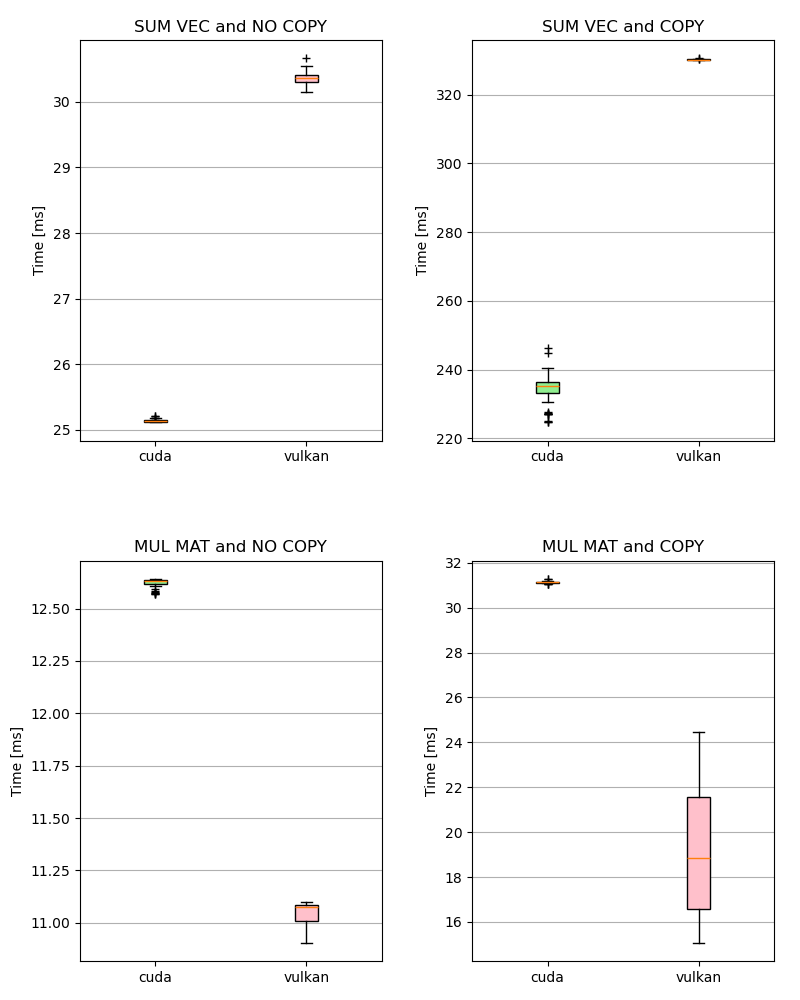
\includegraphics[width=1\linewidth]{images/chapter4/bench_u32.png}
  \caption{Benchmark con uint}
  \label{fig:bench_u32}
\end{figure}

\begin{figure}[ht]
  \centering
  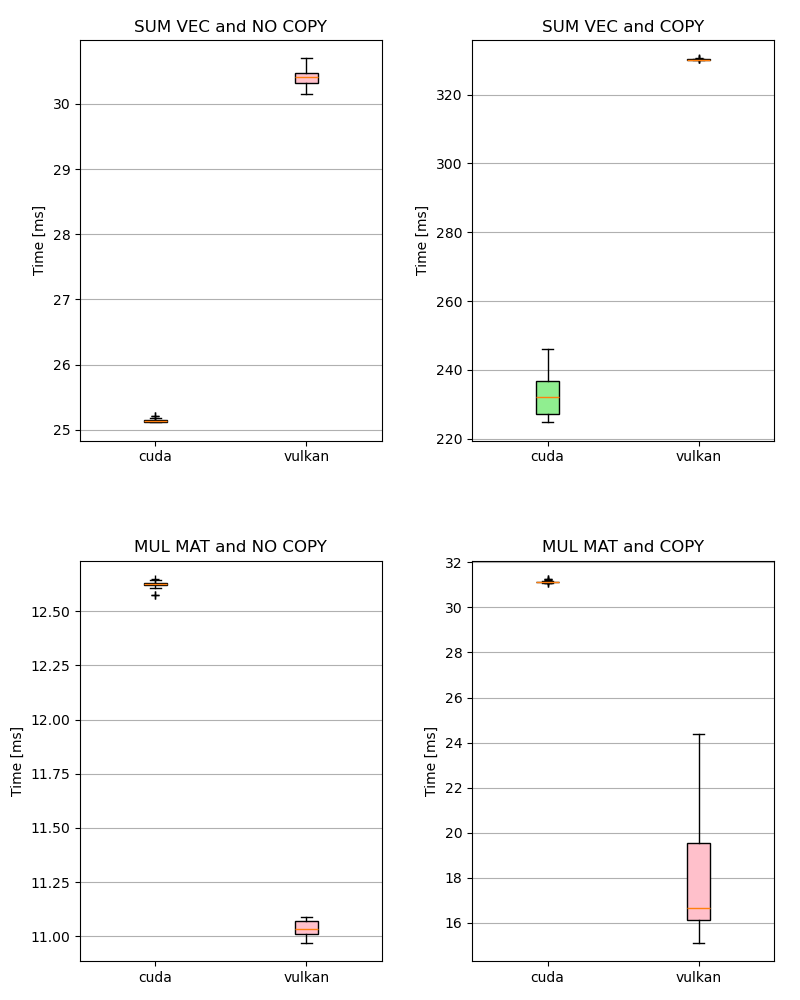
\includegraphics[width=1\linewidth]{images/chapter4/bench_f32.png}
  \caption{Benchmark con float}
  \label{fig:bench_f32}
\end{figure}

\begin{figure}[ht]
  \centering
  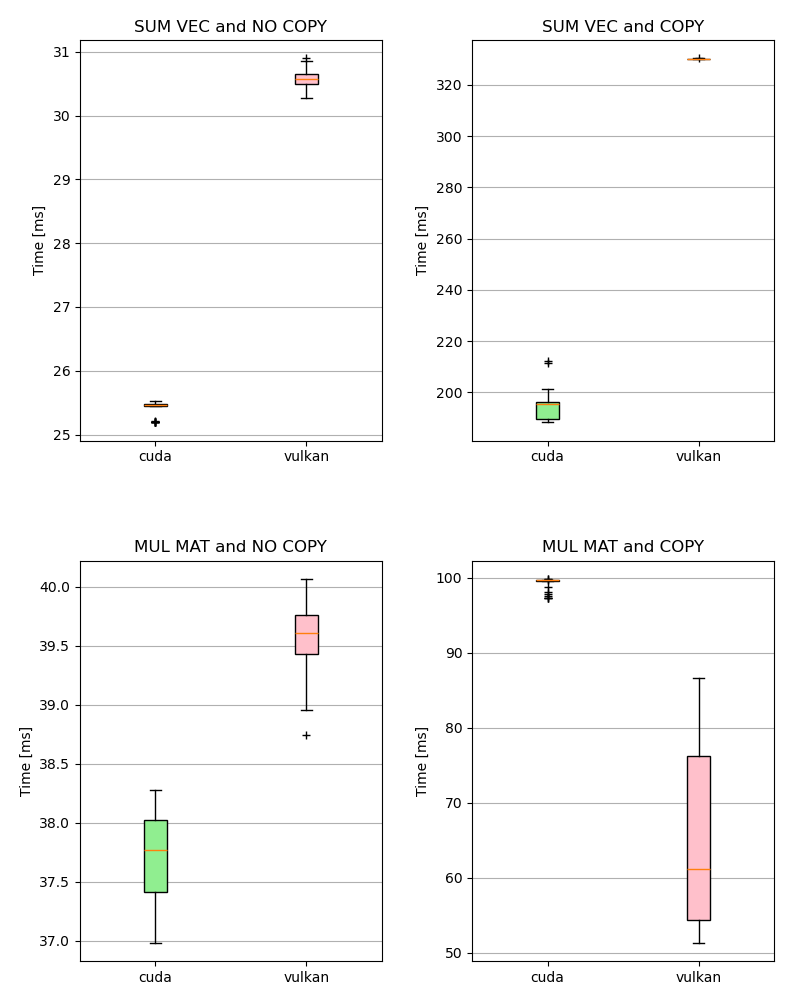
\includegraphics[width=1\linewidth]{images/chapter4/bench_f64.png}
  \caption{Benchmark con double}
  \label{fig:bench_f64}
\end{figure}

Le considerazioni sui risultati ottenuti sono riportate nel prossimo capitolo.